\documentclass{article}
%\usepackage[a4paper, total={6in, 8in}]{geometry}
\usepackage{geometry}
 \geometry{
 a4paper,
 total={210mm,297mm},
 left=20mm,
 right=20mm,
 top=-2mm,
 bottom=2mm,
 }
%\usepackage[margin=0.5in]{geometry}

\usepackage{amsmath,amssymb}
\usepackage{ifpdf}
%\usepackage{cite}
\usepackage{algorithmic}
\usepackage{array}
\usepackage{mdwmath}
\usepackage{pdfpages}
\usepackage{mdwtab}
\usepackage{eqparbox}
\usepackage{cite}
%\onecolumn
%\input{psfig}
\usepackage{color}
\usepackage{graphicx}
\setlength{\textheight}{23.5cm} \setlength{\topmargin}{-1.05cm}
\setlength{\textwidth}{6.5in} \setlength{\oddsidemargin}{-0.5cm}
\renewcommand{\baselinestretch}{1}
\pagenumbering{arabic}
\usepackage{ragged2e}
\renewcommand{\baselinestretch}{1.5}

\begin{document}

\textbf{
\begin{center}
{
\large{School of Engineering and Applied Science (SEAS), Ahmedabad University}\vspace{4mm}
}
\end{center}
%
\begin{center}
\large{B.Tech(ICT) Semester V: Wireless Communication (CSP 311) }\\ \vspace{3mm}
\end{center}
}
\begin{itemize}
\item Group No : 15 
\item Group Members:\\\
        Shyam Patel     (AU1741030) \\
        Ratnam Parikh   (AU1741036) \\
        Dhairya Dudhatra(AU1741058) \\
        Jinesh Patel    (AU1741076) \\
        Nisarg Shah     (AU1741087)     
    
%\item Associated with Project: DST-UKIERI
\item Project Title:
\subitem 1) Impact of Mobility on Physical Layer Security over Wireless Fading Channels 
\subitem 2) Impact of Eavesdropper Mobility on Physical Layer Security over Wireless Fading Channels
\end{itemize} 

\section{Introduction}
\subsection{Background}
\begin{itemize}
    \item 
    A steadily growing component of modern communication systems nowadays is based on wireless technologies that make use of smaller and more mobile and portable electronic devices.The issues of privacy and security in wireless communication
networks have taken on an increasingly important role as these
networks continue to flourish worldwide. Traditionally, security
is viewed as an independent feature with little or no relation to
the remaining data communication tasks and, therefore, state-
of-the-art encryption algorithms are insensitive to the physical
nature of the wireless medium. 
 For a Typical Eavesdropper Scenario. To meet this challenge, system designers have traditionally borrowed cryptography techniques and implemented at the upper layers of the Networks protocol stack. The computational resource-intensive-needy nature of cryptography-based security algorithms however does not scale well when employed in devices which are continuously growing smaller and smaller in size and have reduced and lower power constraints. Lighter weight security implementations are needed for this new generation of smaller devices, especially as the development of Internet of Things devices continues at an ever-increasing rate. Physical Layer Security is a collection of different security techniques that seek to exploit the random nature of wireless channels to either obscure the information being exchanged over the channel and/or provide a mechanism to generate private keys that can then be used to facilitate encrypted communications
    Thus need to provide a light-weight security strategy for these systems has become a more important problem. While the underlying techniques of PLS(Physical Layer Security) have been known for some time, the potential secrecy benefits of them need further investigation.The need to deliver secure communications utilizing wireless systems is an increasingly complex challenge given both the broadcast nature of the wireless medium and the rapid advancements in technology available to potential eavesdroppers. 
\item    
During the past decades,
physical layer security has been widely investigated since
Wyner proposed the wiretap channel model [1]. For Rayleigh
fading wiretap channel, the secrecy outage probability (SOP)
was defined and the ergodic secrecy capacity [2] [3] was
considered to describe the average secrecy capacity when the
eavesdropper’s channel state information (CSI) is unknown to
legitimate users. Recently, there has been a growing interest
in studying the impact of large scale path loss and small
scale channel fading on physical layer secrecy [4-9]. The
challenge in taking the path loss factor in consideration for
the physical layer secrecy lies in that the location of the passive
eavesdropper is unknown to legitimate users. The stochastic
geometry theory [10] is used as an effective mathematical tool
to model the random location and the number of nodes (i.e.,
legitimate and eavesdropping nodes) in the networks [4-9].
\item 
For the networks with random mobile nodes, [11] derived
the probability density distribution function (PDF) of the
received power under the Random Way point Model [12] and Random Direction RD mobility [13]
models. The authors derived the mathematical expressions for
path loss exponent of 4 in terms of confluent hyper geometric
function. In [14], the authors derived the outage probability
and average bit error rate (BER) for RWP mobile nodes
under the Nakagami-m fading channel. However, all these
works only studied received signal quality in random mobile
networks [11], [14]. The impact of mobility on physical layer
security has not been well studied.
\end{itemize}

\subsection{Motivation}
%Write one paragraph which \textbf{clearly indicates the work/condition/scenario that has not been considered in the literature till date,} which motivates you to carry out this work.
    
    Most existing work study physical layer secrecy with static Eavesdropper or mobile/static legitimate User and Proper Knowledge of CSI\textbf{(Channel State Information)} or Perfect CSI at Receiver side.The distance of Eve to Base station was assumed to be fixed and Time-invariant.Though in many scenarios of Wireless network Eve can be mobile e.g., People sharing ride with you in cab,bus or People normally walking along the street.So Mobility of Eavesdropper is the case which needs to studied.
    %Also,Perfect CSI is assumed at Legitimate user(Receiver side) which does not happen in real life scenarios of Wireless network.so    
    \subsection{Contributions}
\begin{itemize}
\item Justify contribution-1 in detail
\newline
The project is related to the effect of mobility on physical layer security. Here, in the base article the effect of mobility of legitimate user is taken into consideration. For new analysis we have also tried to bring in the effect of mobility of eavesdropper. The SPDF of the mobile eavesdropper is now taken into consideration. The SPDF is taken to be the same as that of mobile user which is specific for the Random Mobility Model(RWP) used in base article and our new analysis as the base system model.
\end{itemize}

%are Once accomplished,we can improve sensing performance based on  the knowledge of channel statistics. Further, for more realistic considerations we would extend the above setup to SIMO, MISO and MIMO system models. The performance metrics would be the statistical properties like idle/busy period durations, its mean, variance and Occupancy rate(or duty cycle) of Primary user (PU). The metric for spectrum sensing would be detection probability $(P_d).$ Also the estimation error varies as per sensing period$(T_s)$ and thus KS distance would be an additional metric to be taken into consideration. 
	%\vspace{8cm}
\section {Performance Analysis of Base Article}
\begin{itemize}
\item List of symbols and their description


\begin{table}[h]
 \centering
% \caption{List of notations used}
 
 \begin{tabular}{|c|c|}
 \hline
 \textbf{Symbol} & \textbf{Description}                                     
 \\ \hline
$ P(C_s > 0)$        & Positive Secrecy Capacity Probability (PSCP)          
\\ \hline
$ P^{out}_{R_s}$        & Secrecy Outage Probability (SOP)   
\\ \hline
 $f(d)$          & Spatial node distance Probability Density distribution Function (SPDF)  
 \\ \hline
 $R_E^{Guard}$ & Secrecy guard zone 
  \\ \hline
   $P_T$ & Transmit Power 
  \\ \hline
   $a$ & path loss co-efficient 
  \\ \hline
   $\bar d_{AB}$ and $\bar r_E $ & Normalized distances 
  \\ \hline
     $ R_s $ & desired Secrecy Rate 
  \\ \hline
  $ \epsilon,\epsilon1,\epsilon2,\epsilon3 $ & Parameters for SOP  
  \\ \hline
  $ R_s $ &   the power to radius ratio with exponent 
  

  \begin{tabular}[c]{@{}c@{}} 
 
 \end{tabular}                                                                      \\ \hline
 \end{tabular}
 \end{table}

\item \textbf{System Model/Network Model} : Insert the image of system model used in your base article and/or in your new work and clearly describe the channel, the transmitted signal (e.g BPSK,QAM etc.,) and the nature of noise.
\\
The model is illustrated in Fig. 1. We consider three single
antenna ends in a circular area with radius R. Alice is the BS
or AP located in the center of the circle, communicating with
the legitimate user Bob. A passive eavesdropper Eve is located
somewhere in the circular region. The legitimate users (Alice
and Bob) do not know the exact location of Eve. During the
communication period, Bob moves randomly in the circular
area. The mobile track of Bob is random and the distance
between Bob and Alice is time-varying. We study the secrecy
of the mobile receiver under three typical random mobility
models [15], [12], [13], which are illustrated below. \\
\textbf{RWP mobile Bob:} First, Bob randomly starts from point $D_0$
in the circular region. Then, he randomly chooses a coordinate
$D_1$ ($D_1$ is uniformly distributed in the circular area) as his next
destination point and moves to it with a constant speed $v_1$. The
speed can be randomly (uniformly) chosen from [ $v_{min}$ , $v_{max}$ ].
After Bob arrives at the destination point $D_1$, then he may
choose to stop for a random pause time $t_{p,1}$ at this point.
$t_{p,1}$ (i = 1, 2, 3...) is randomly chosen from [$t_{p,min}$ , $t_{p,max}$ ].
Then, he chooses a new destination $D_2$ and moves to it with a
new speed $v_2$, and continues this process. The RWP mobility
model is a very good model for real world mobile users in a
specific region. 

\textbf{RD mobile Bob} : First, Bob randomly starts from point $D_0$
in the circular region. Then, he randomly chooses a direction
$\theta_1$ (0 $\geq$ $\theta_1$ $\geq$ 2$\pi$) and moves with a constant speed $v_1$ ($v_{min}$ $\geq$
$v_1$ $\geq$ $v_{max}$ ) for a random period of time $t_1$ ($t_{min}$ $\geq$ $t_1$ $\geq$ $t_{max}$ ).
He may pause for a random time $t_{p,i}$ ($t_{p,min}$ $\geq$ $t_{p,i}$ $\geq$ $t_{p,max}$ ).
Then, he chooses a new direction $\theta_2$ and moves to it with a
new speed $v_2$ under a new travel time $t_2$ , and continues this
process. Obviously, the RD Bob may dash on the border of
the region. Many works have studied the rebound effect on
the region border and here we assume Bob rebounds with a
new direction $\theta_i = \theta_i + \pi/2$ mod 2$\pi$ at the border [30].\\

\textbf{Eavesdropping model:} Assume that Alice employs a secrecy guard zone with radius $R_E^{Guard}$ [12] to guarantee Eve’s distance $r_E \leq R_E^{Guard}$ to her. This guard zone can be realized
in practice when the antenna of the BS is mounted on a big
tower or roof of a building, where an attacker cannot easily
get close to it.
Firstly, we consider the typical down-link connectivity, when
Alice transmits secrecy data to Bob. We assume Eve knows
Alice’s location and the secrecy guard zone $R_E^{Guard}$ . In the
worst case, Eve can always eavesdrop at the boundary of
the guard zone where the distance between Eve and BS is
$r_E$ = $R_E^{Guard}$ (Eve can be static or move around the guard
zone). This model is illustrated in Fig. 1. Next, consider
the up-link connection, where Bob transmits secrecy data to
Alice. Here we assume Bob can also have a secrecy guard
zone with radius $R_E^{Guard}$ to prevent Eve from approaching
too close to him. The eavesdropping signal quality for Eve
from Bob is related to her distance from Bob. In the worst
case scenario, we assume Eve can always follow Bob with
distance $r_E$ = $R_E^{Guard}$ . Based on this observation, the up-link
and down-link connections are considered symmetric. Without
loss of generality, we only analyze the down-link connectivity
in the rest of this paper.\\\\
   \begin{figure}[htp]
    \centering
    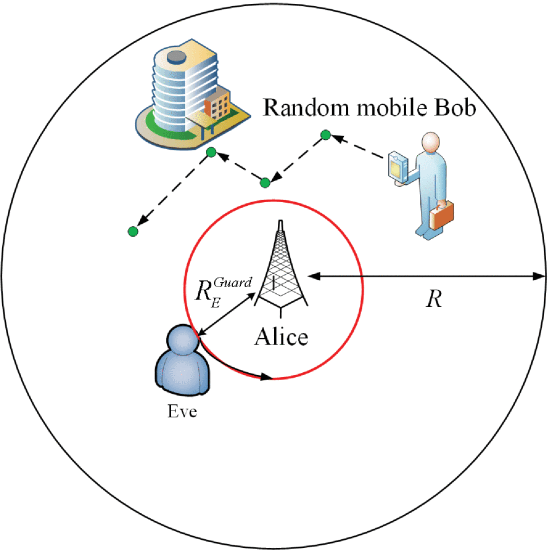
\includegraphics[width=6cm]{Image_11.JPG}
    \caption{}
    \label{fig:}
    \end{figure}
\newpage
\item Detailed derivation of performance metric-I
    
\begin{figure}[htp]
    \centering
    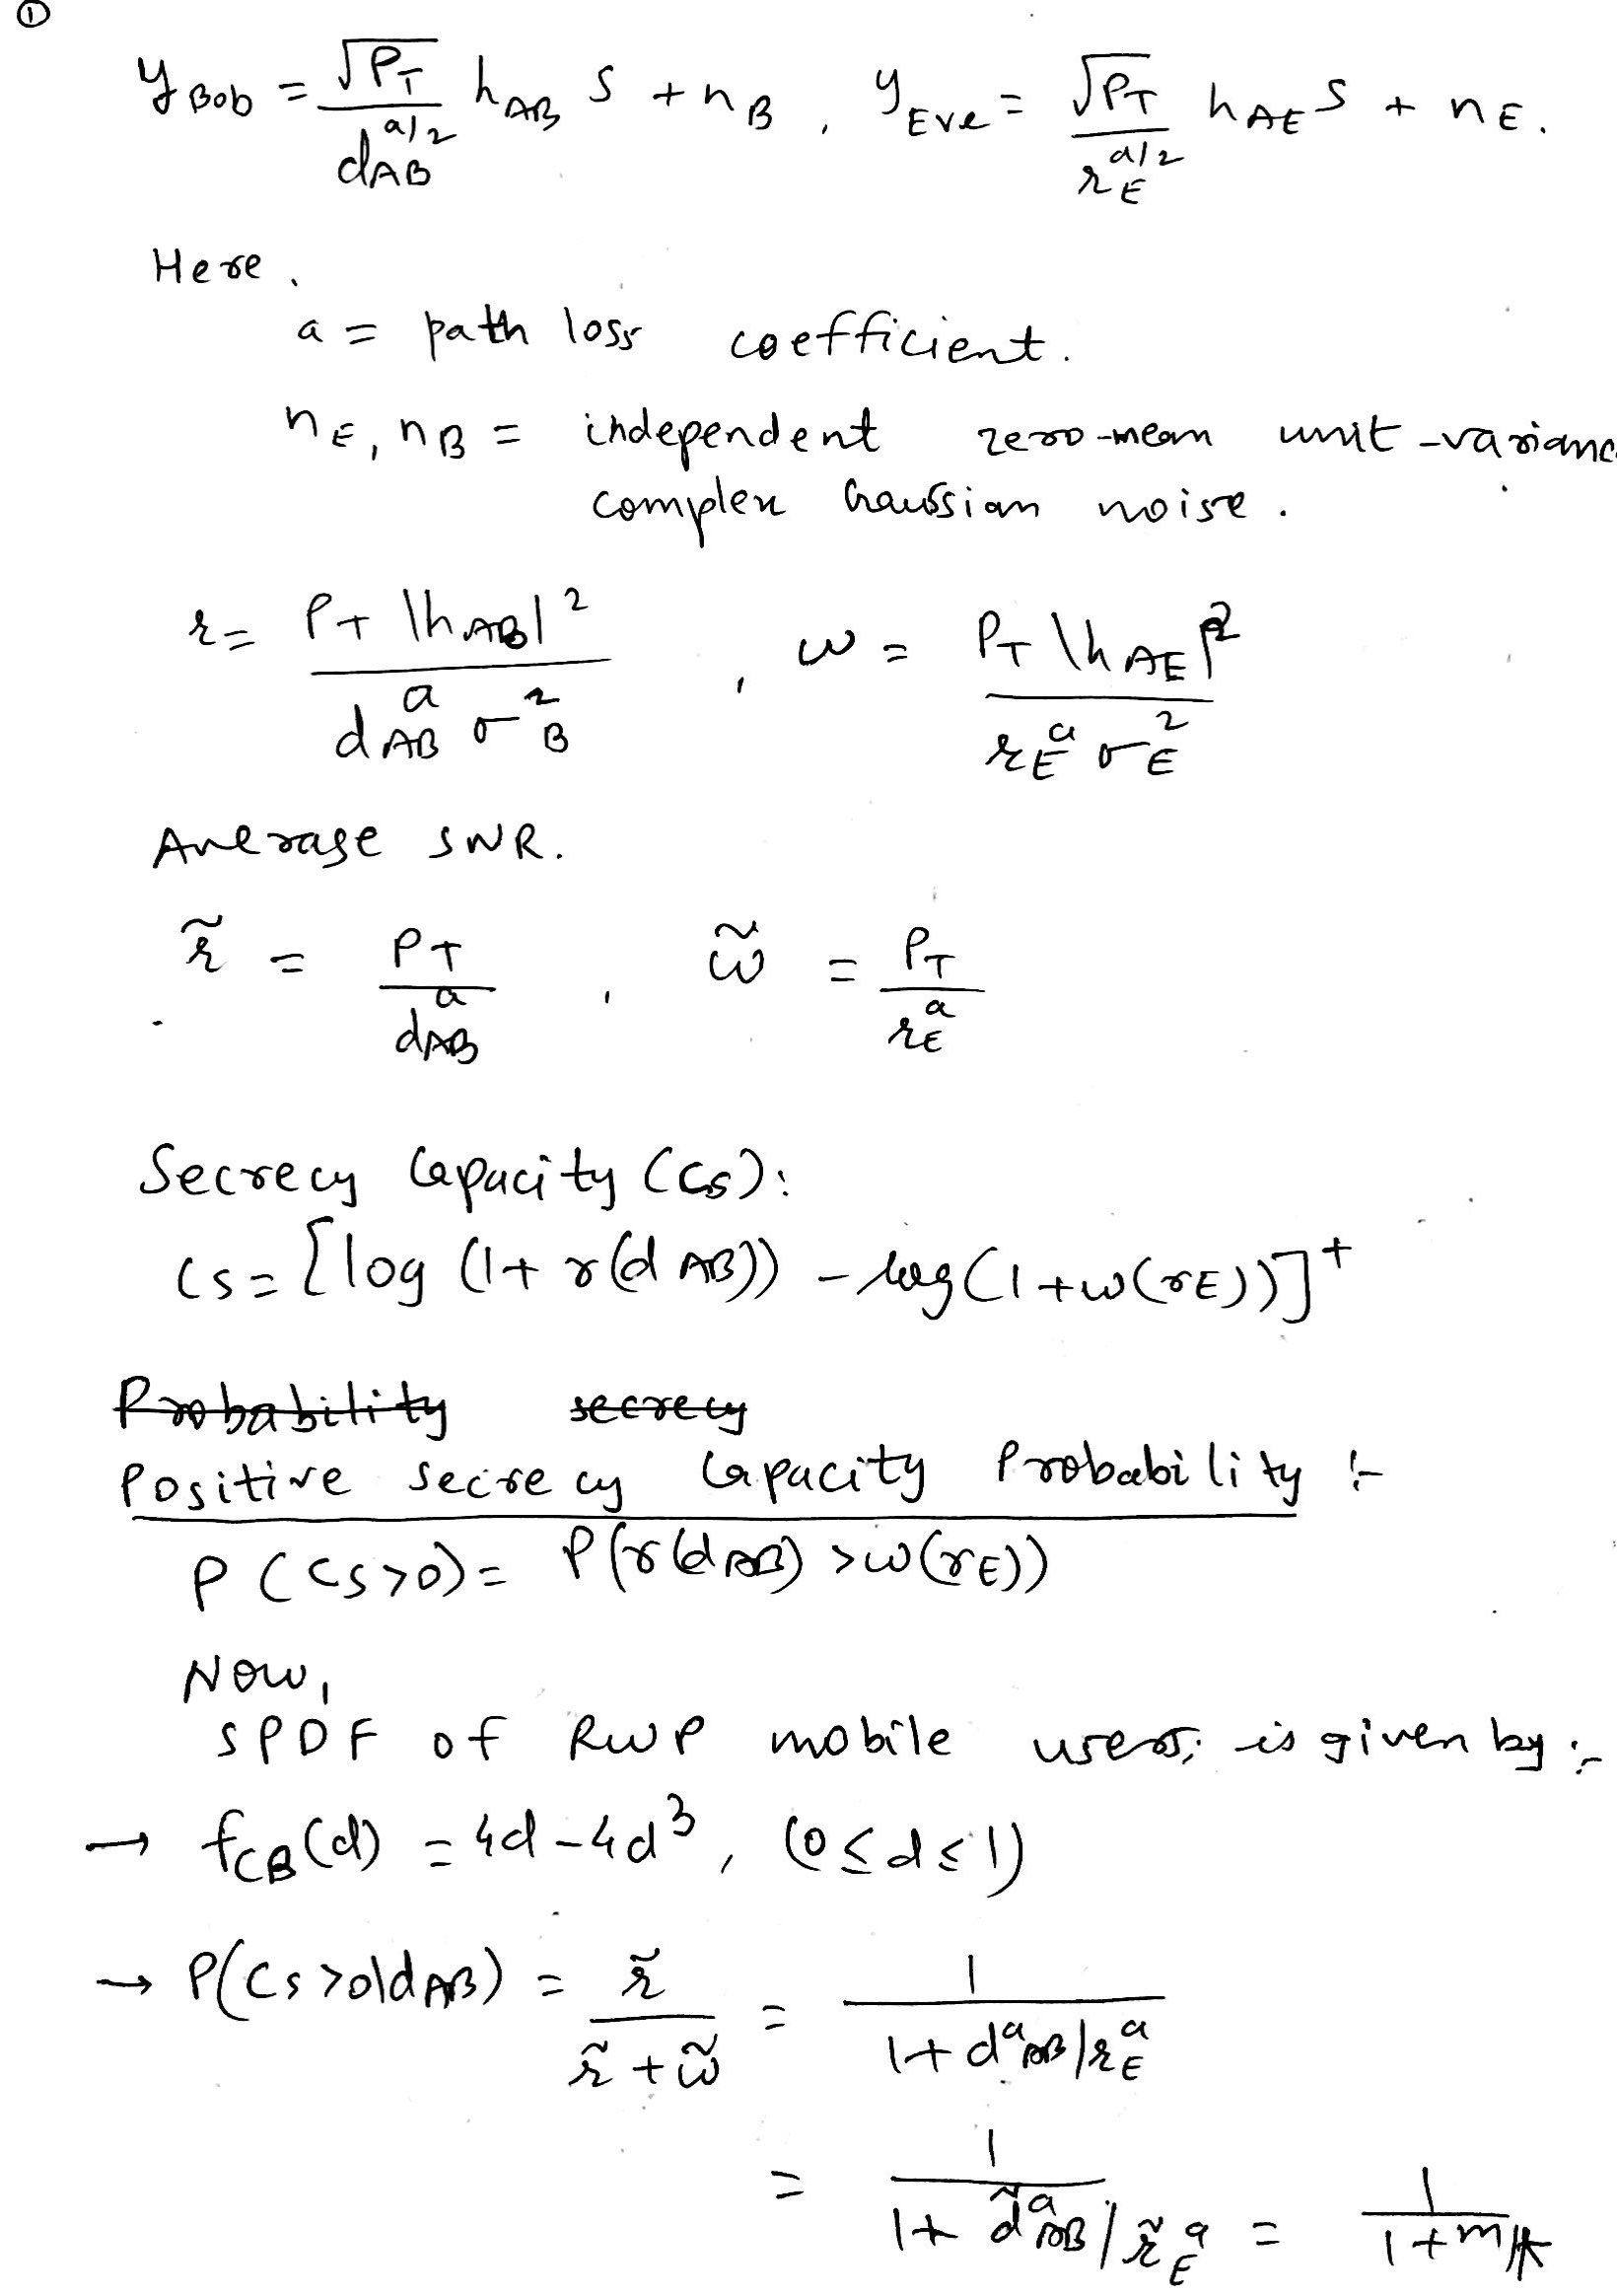
\includegraphics[width=12cm]{Analytical_1_1.jpg}
    \caption{}
    \label{fig:}
\end{figure}
\begin{figure}[htp]
    \centering
    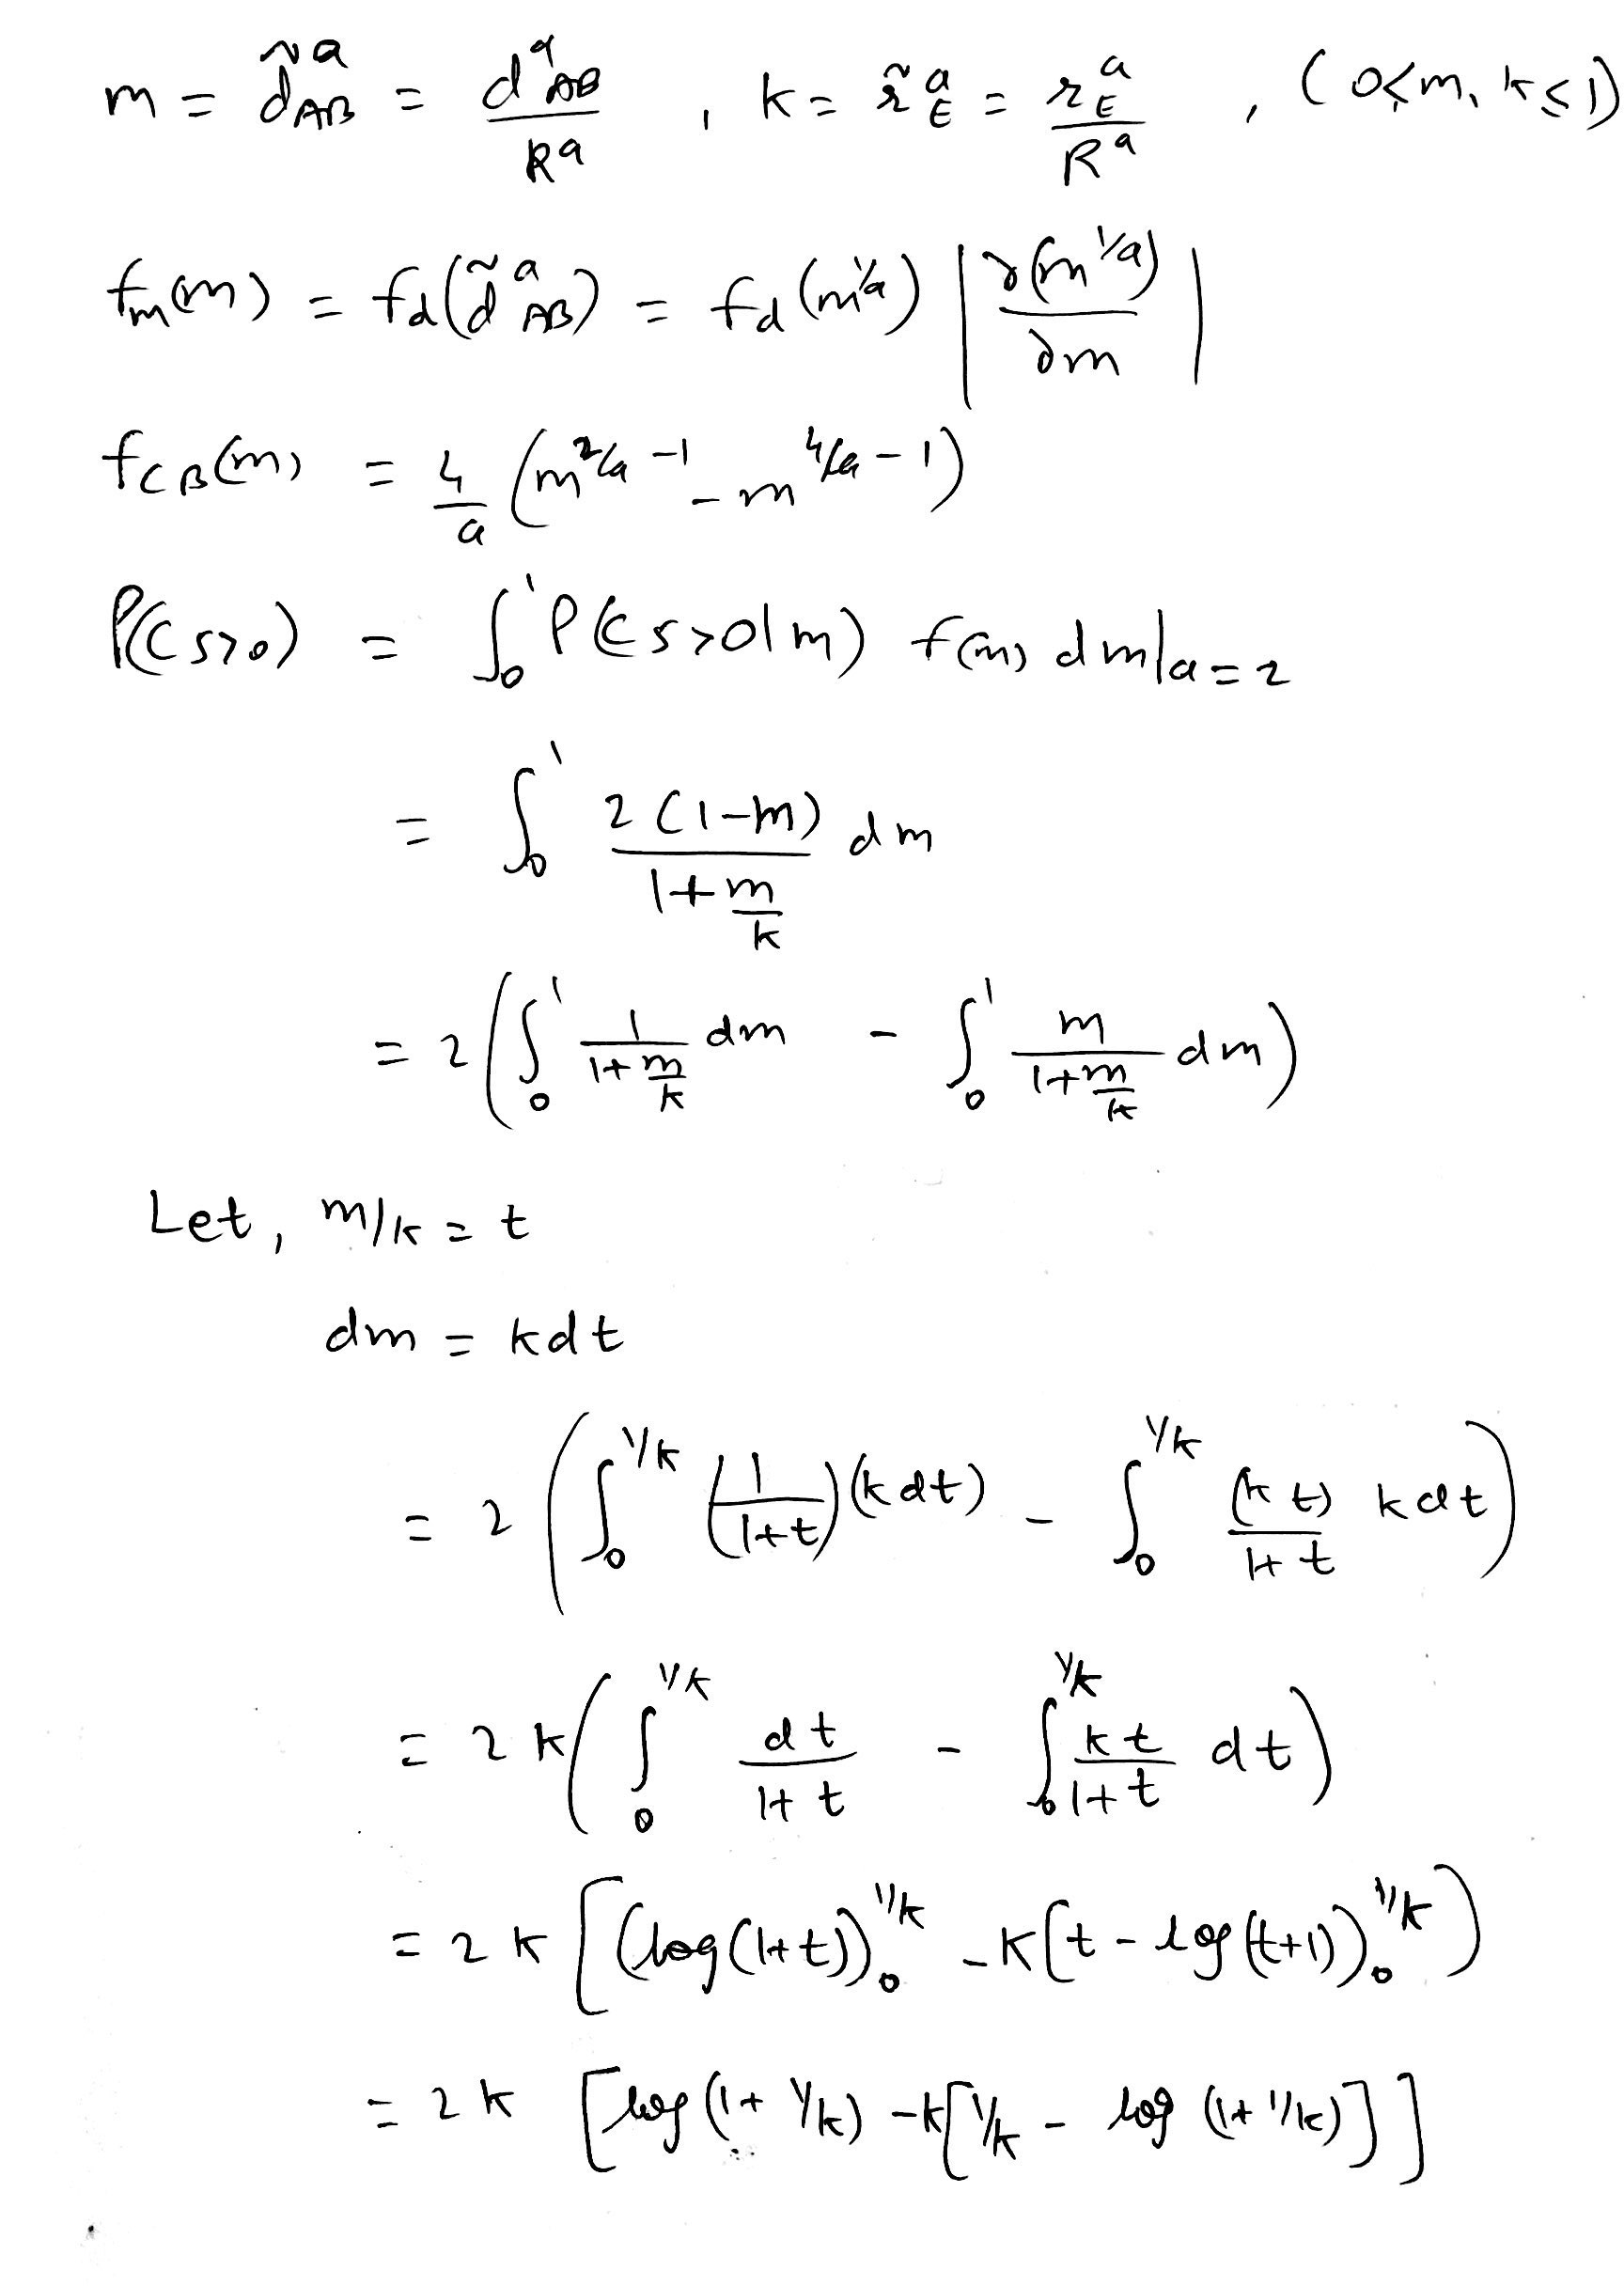
\includegraphics[width=13cm]{Analytical_2_1.jpg}
    \caption{}
    \label{fig:}
\end{figure}
    
    \begin{figure}[htp]
        \centering
        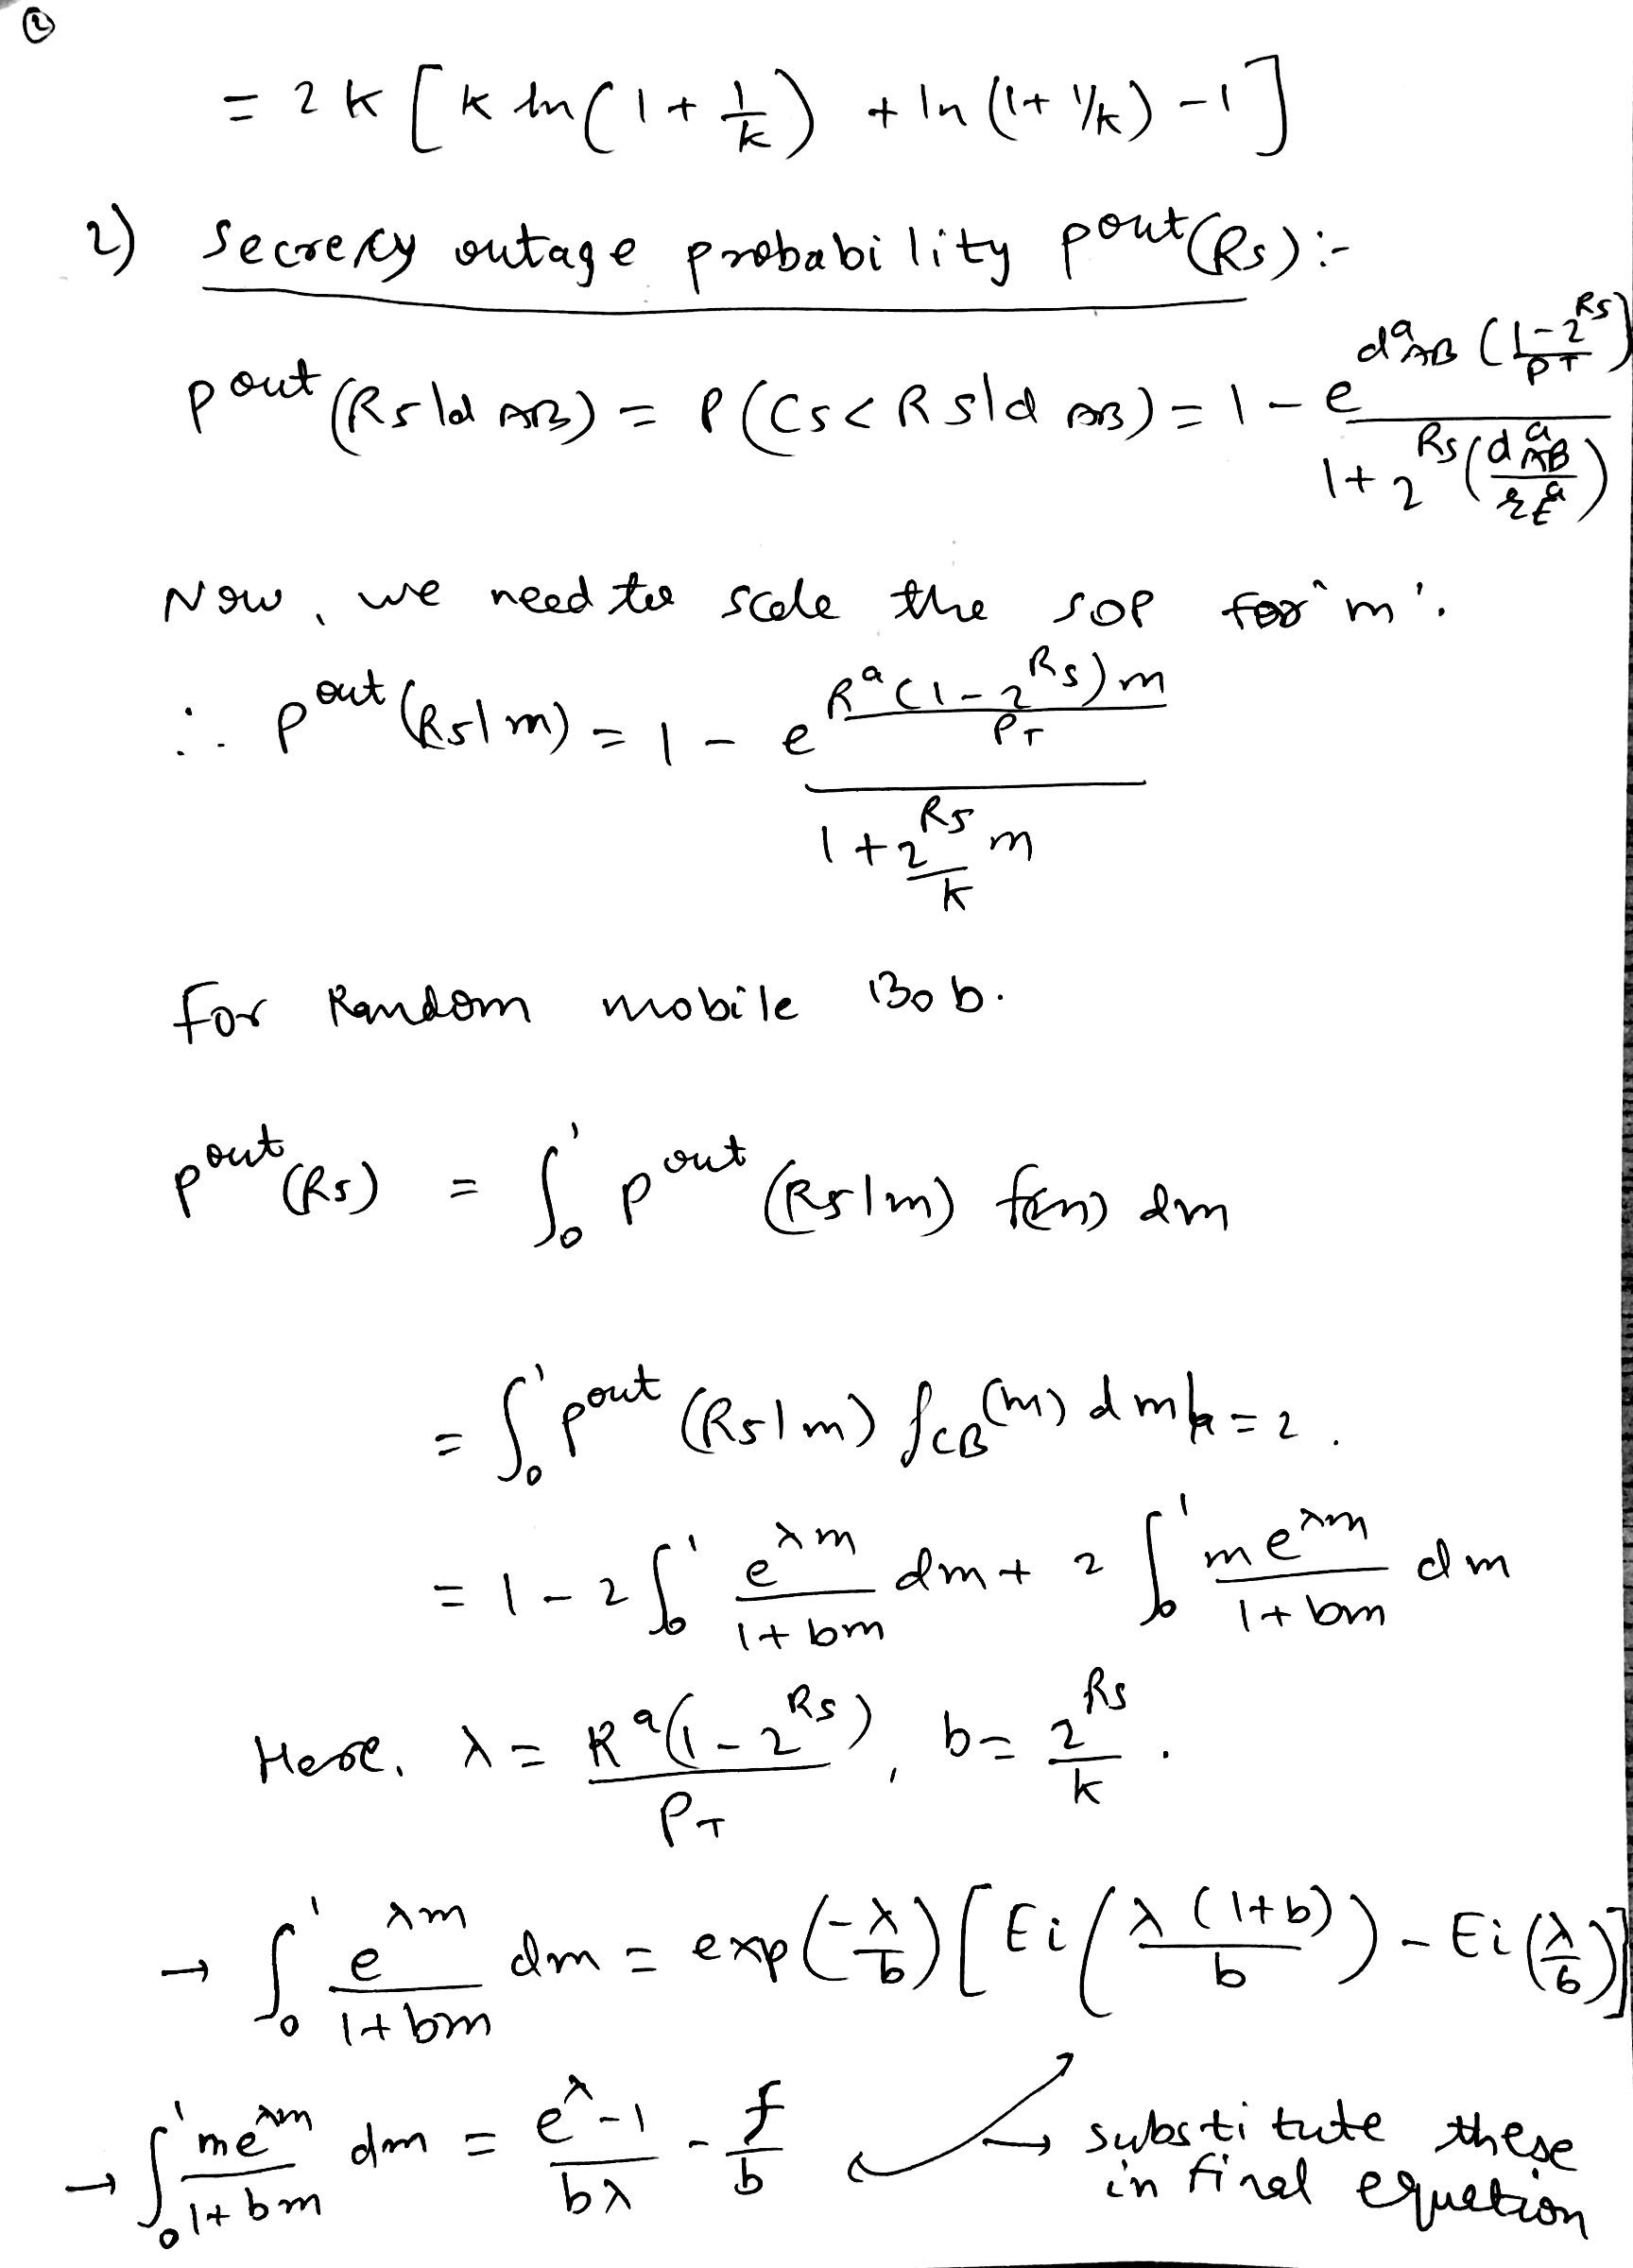
\includegraphics[width=11cm]{Analytical_3_1.jpg}
        \caption{}
        \label{fig:}
    \end{figure}
    \begin{figure}[htp]
        \centering
        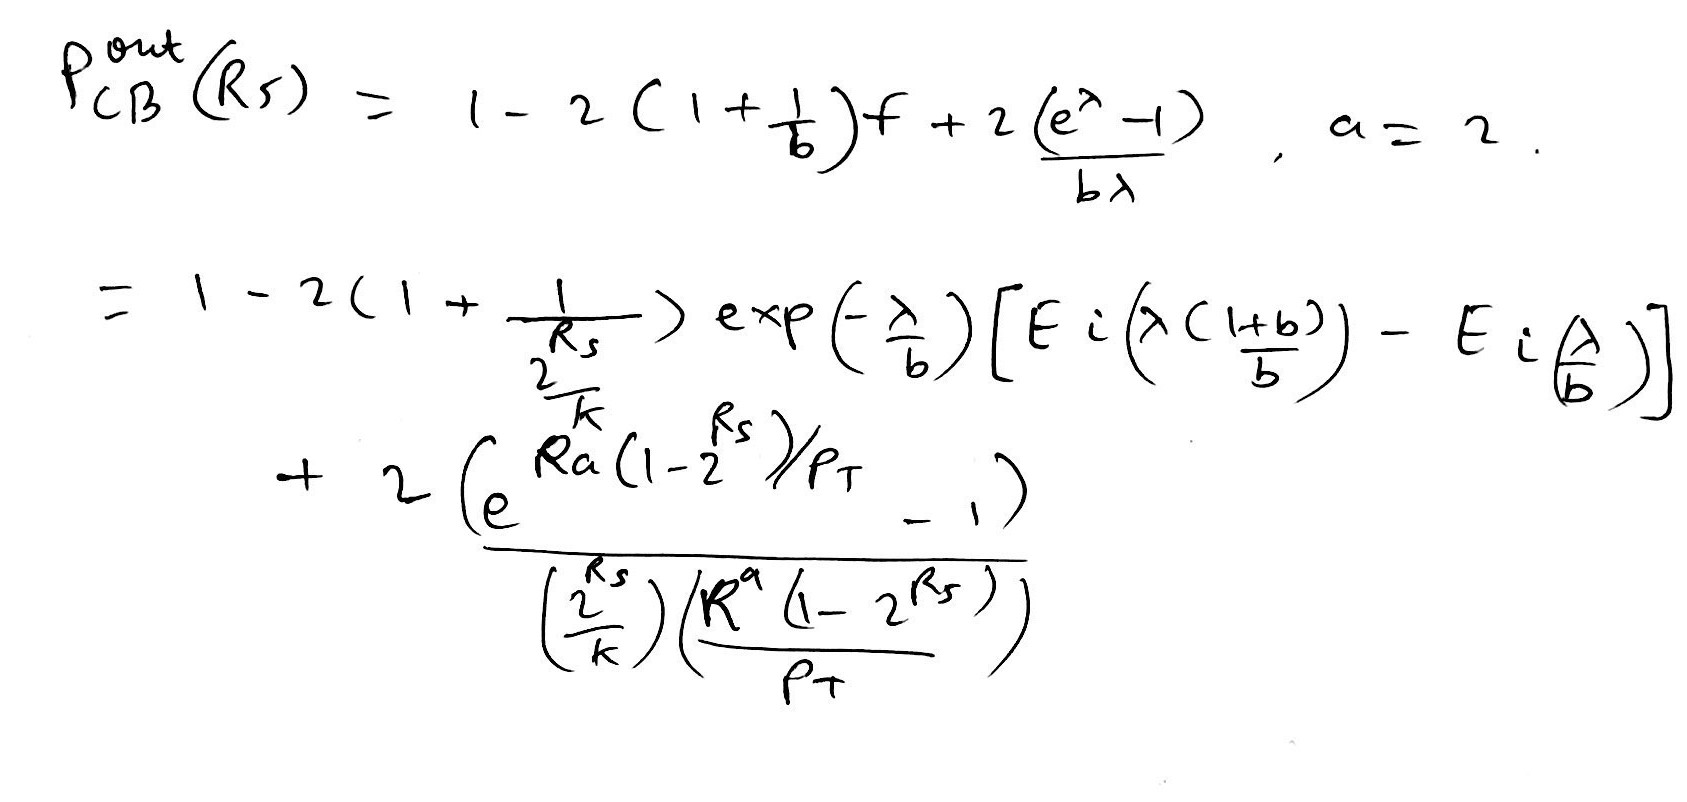
\includegraphics[width=10cm]{Analytical_4_1.jpg}
        \caption{}
        \label{fig:}
    \end{figure}
\end{itemize}

\newpage
\section {Performance Analysis of New contributions}
\begin{itemize}
\item System Model :- RWP Model \textbf{Mobile Bob} and \textbf{Mobile Eve}
\item Detailed derivation of performance metric-I \\
    \begin{figure}[htp]
        \centering
        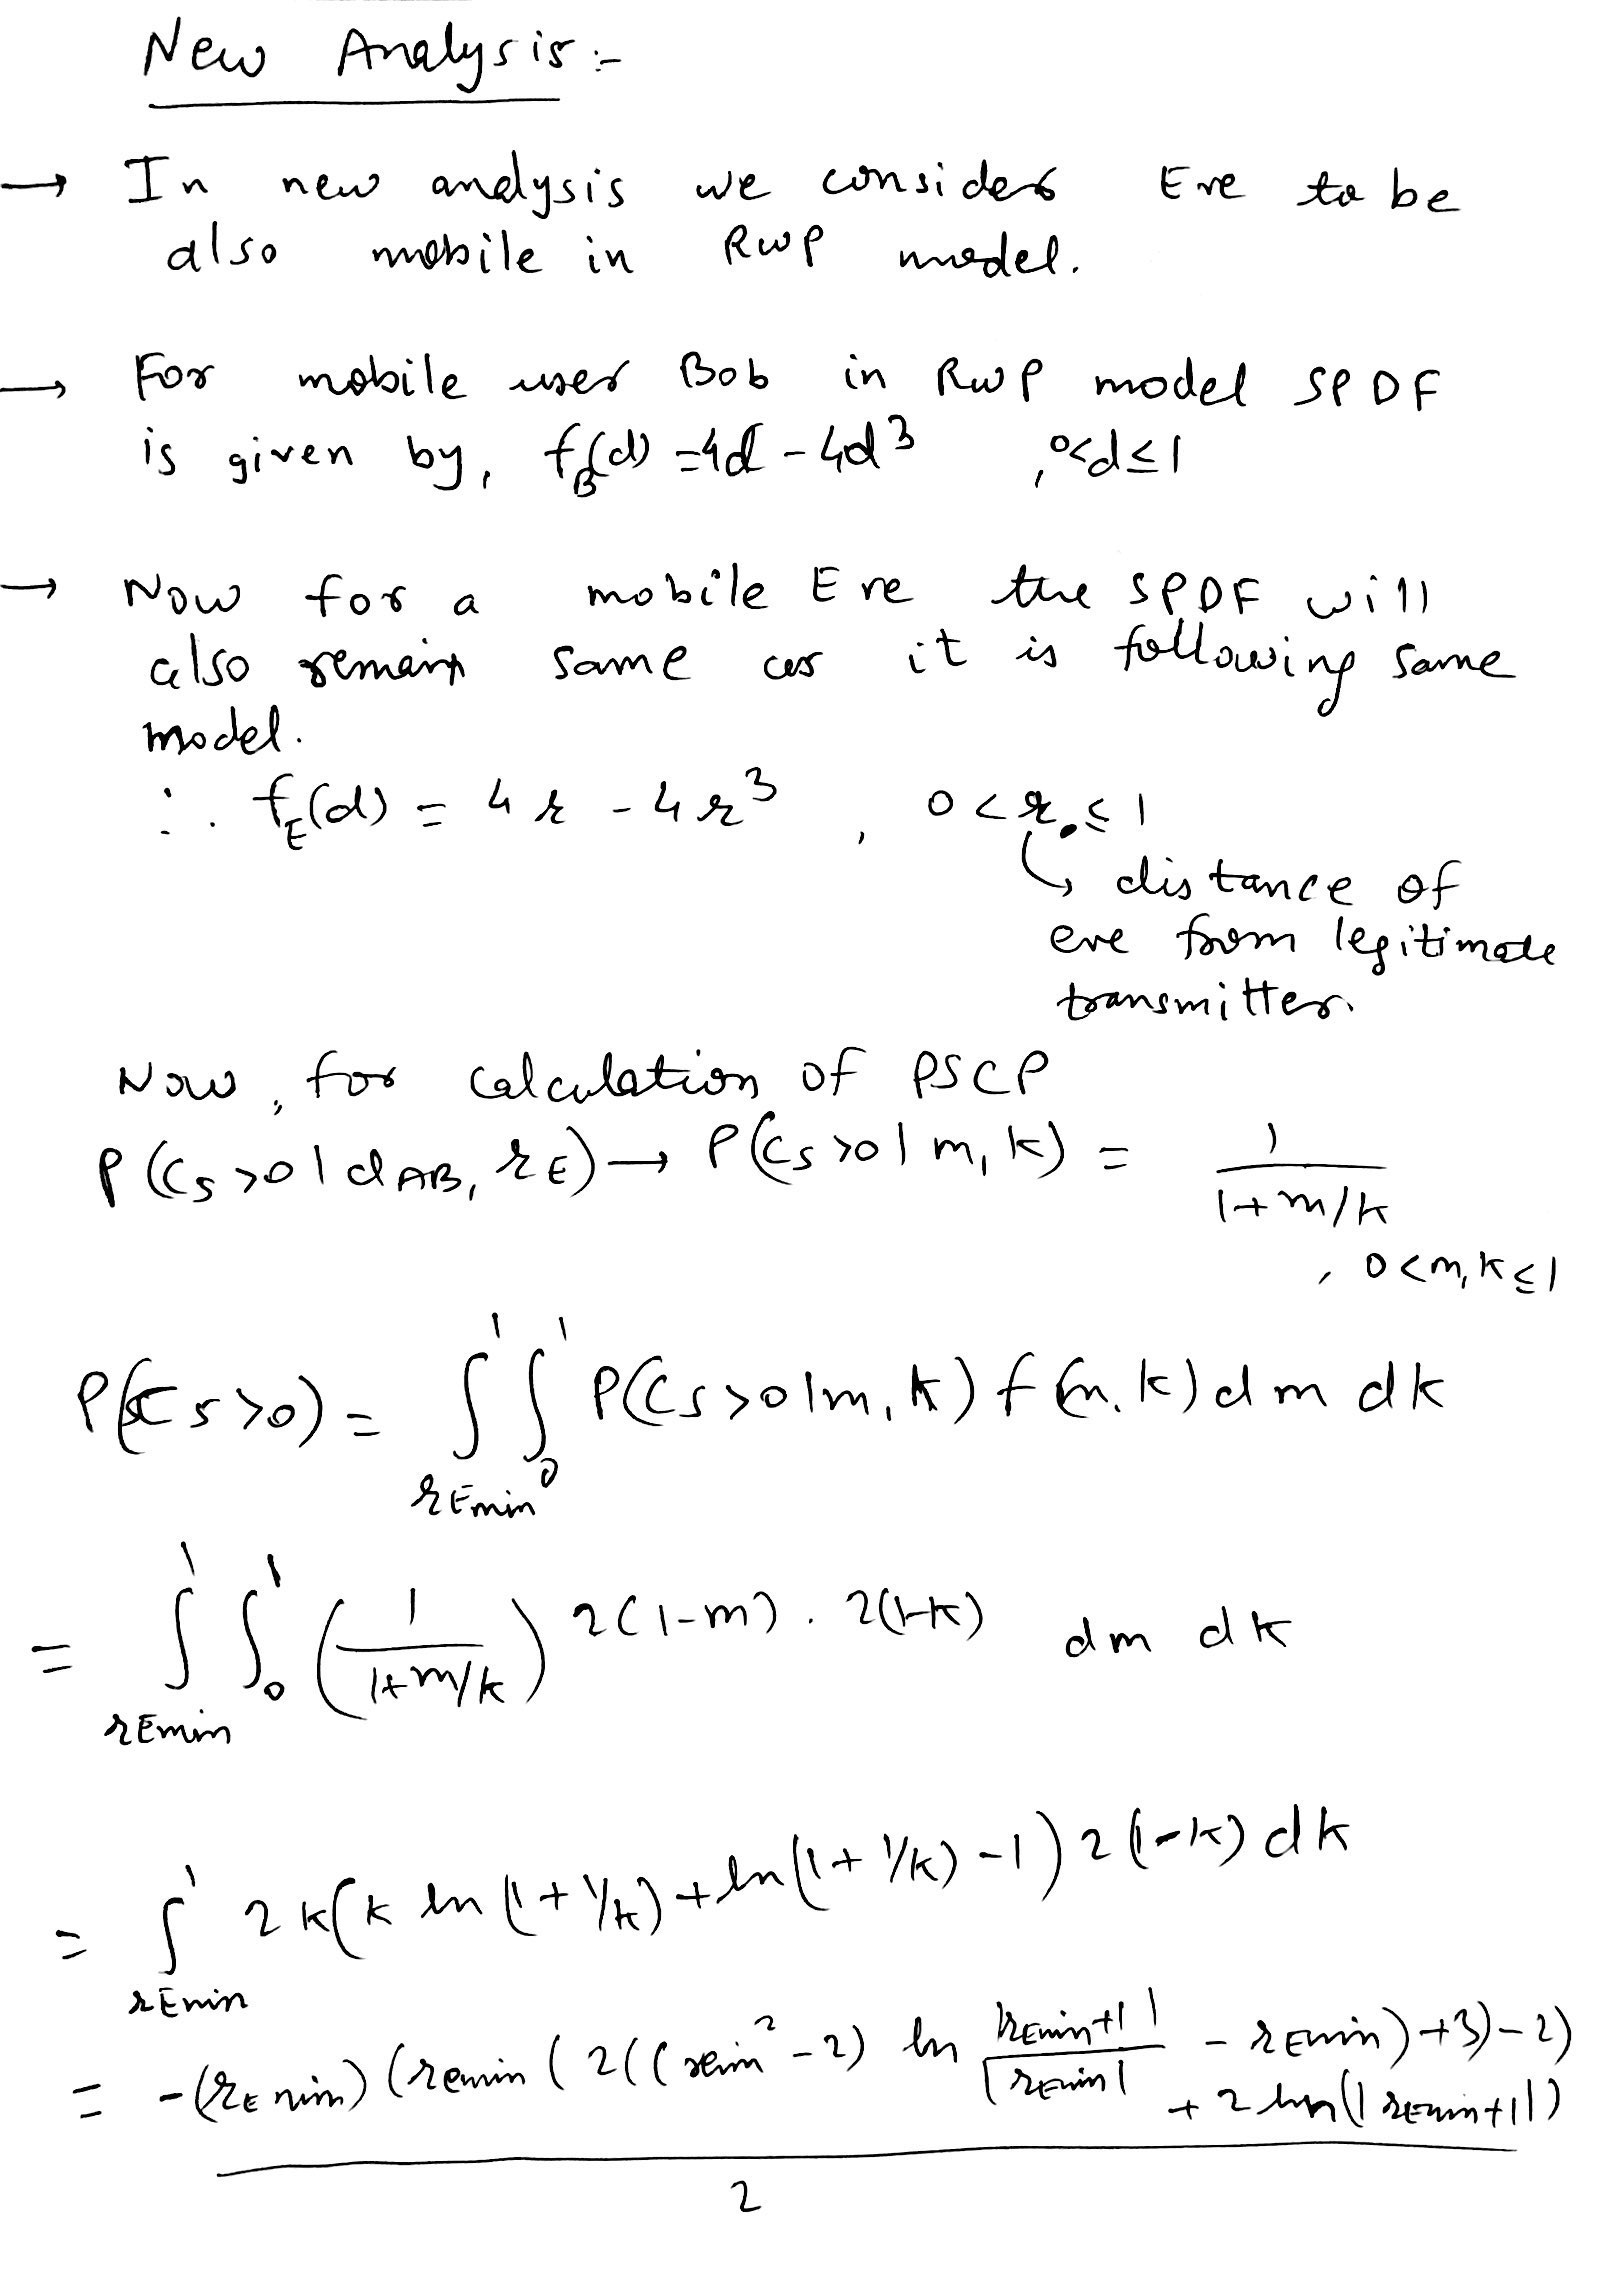
\includegraphics[width=12cm]{new1_1.jpg}
        \caption{New Analysis-1}
        \label{fig:my_label}
    \end{figure}
    \begin{figure}[htp]
        \centering
        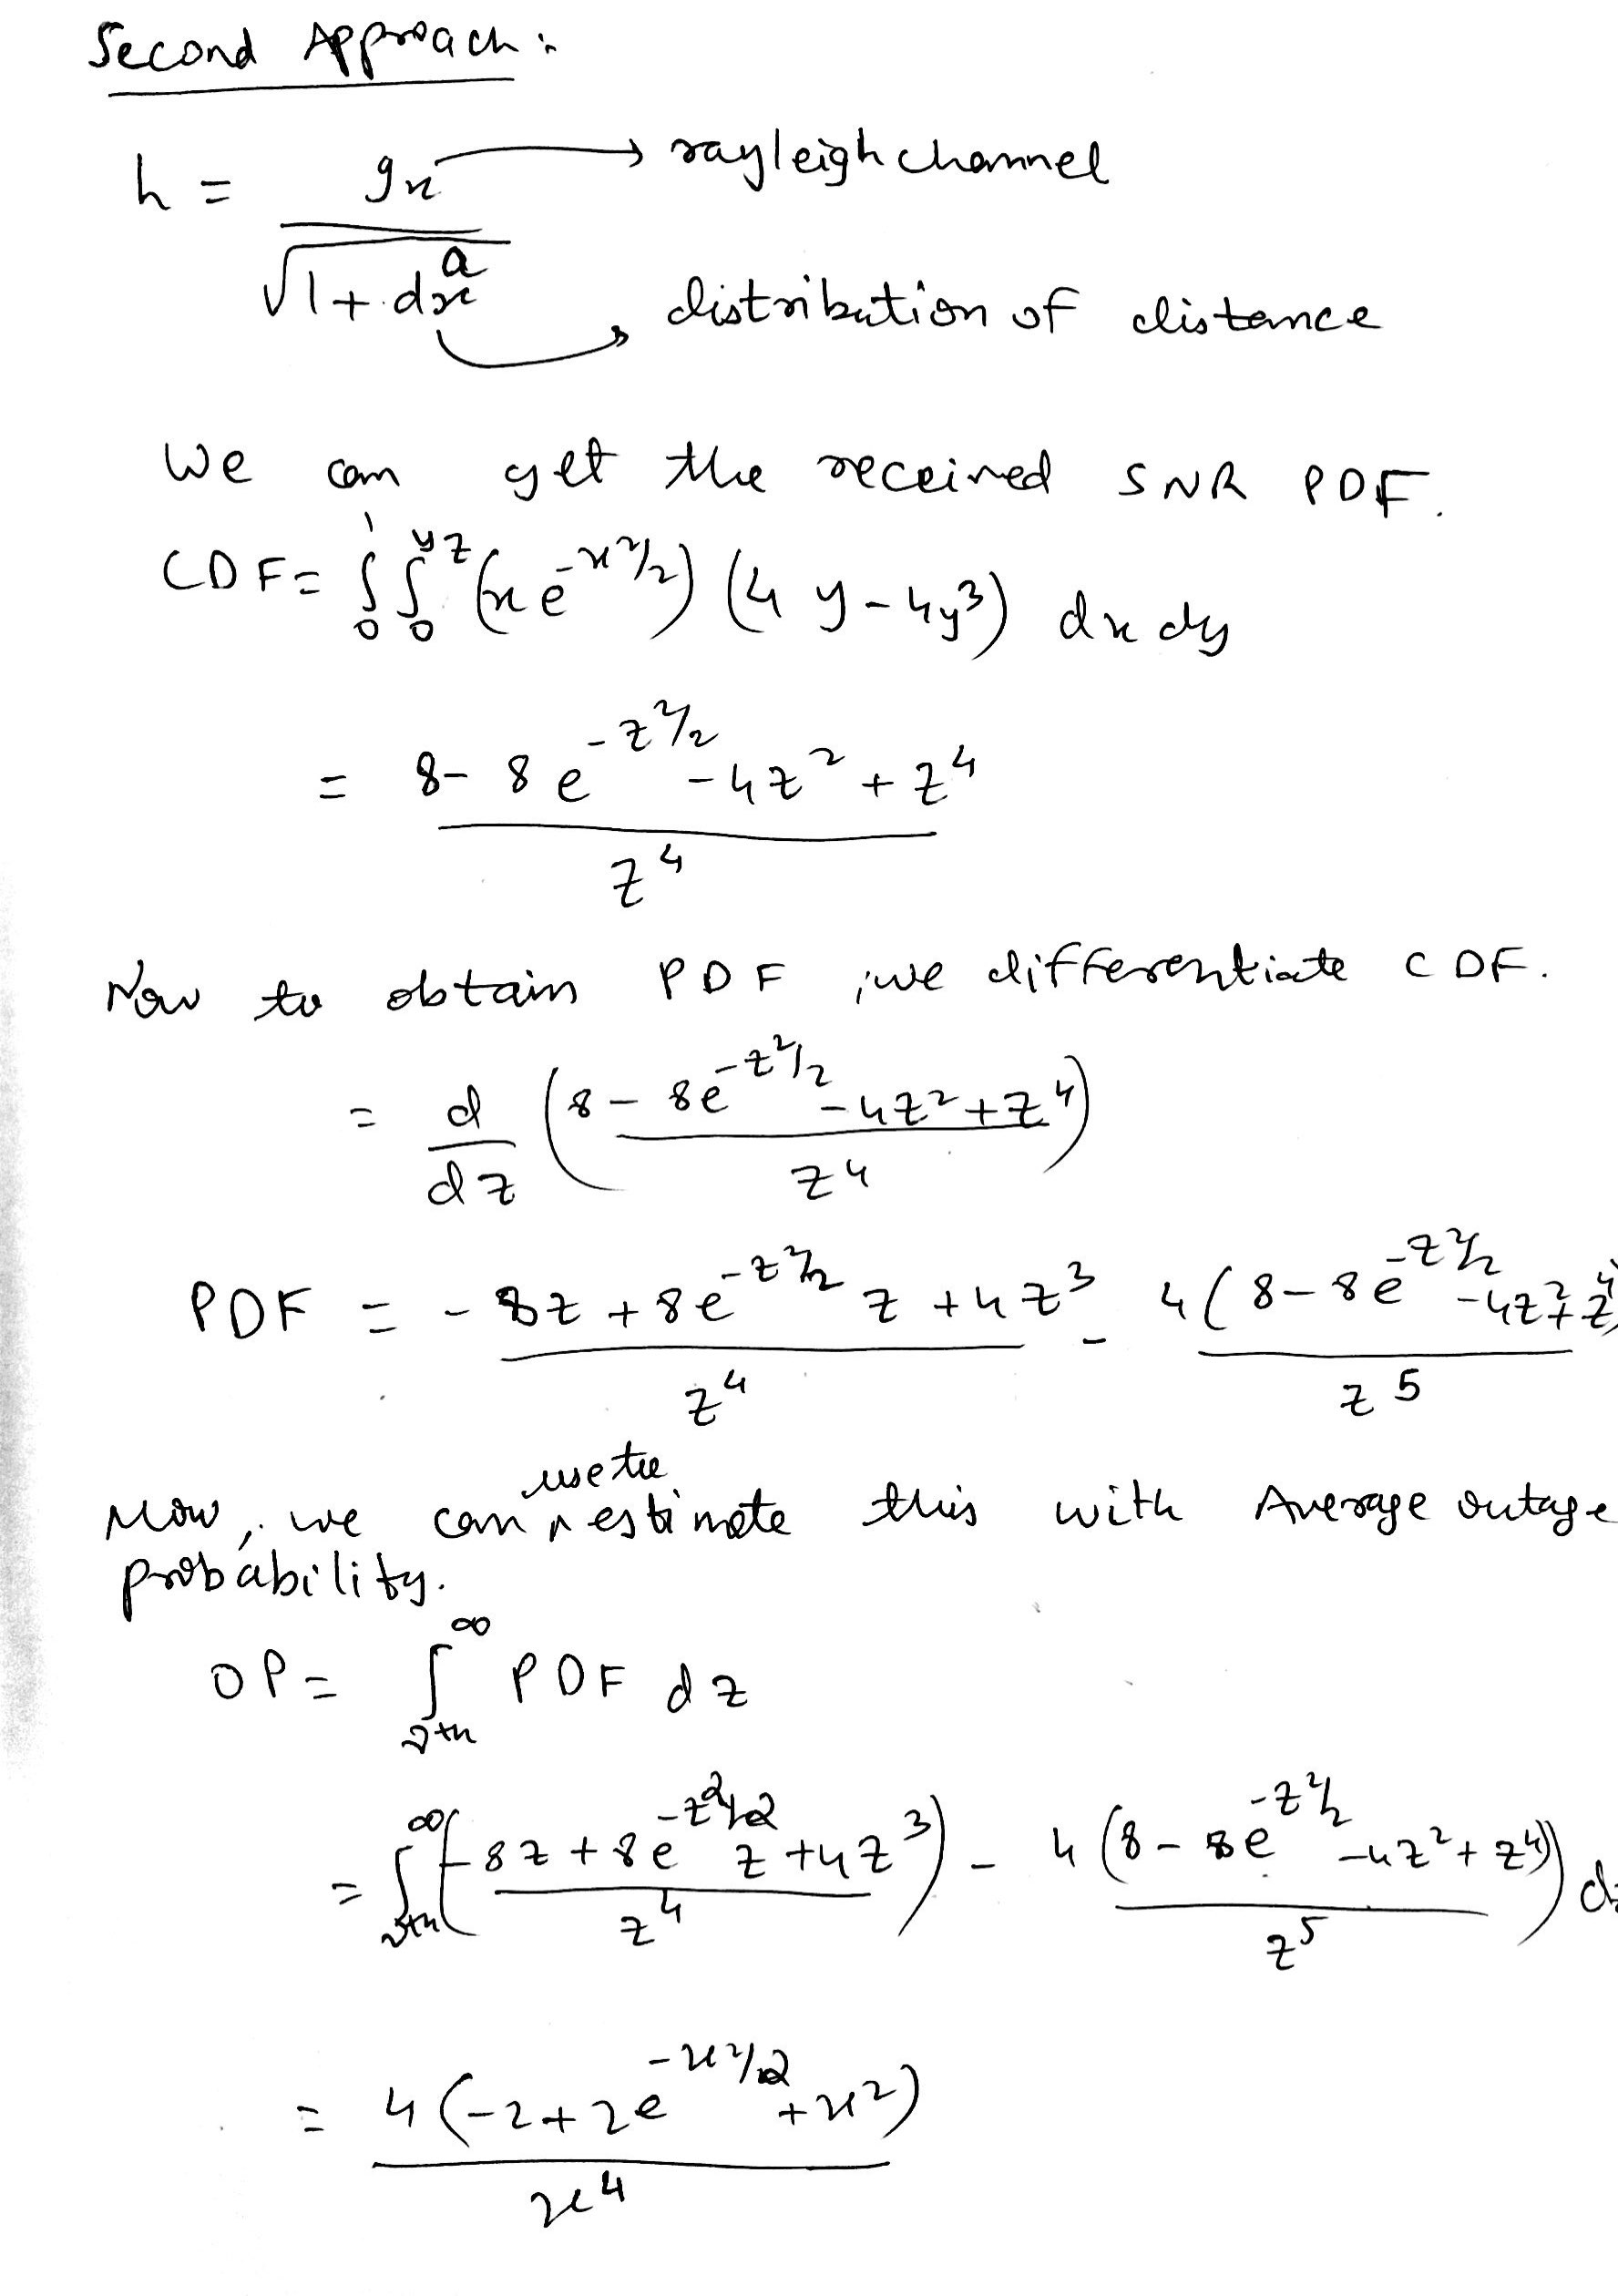
\includegraphics[width=13cm]{new2_1.jpg}
        \caption{New Analysis-2}
        \label{fig:my_label}
    \end{figure}
    
     \begin{figure}[htp]
        \centering
        \includegraphics[width=13cm]{new3_1.jpg}
        \caption{New Analysis-3}
        \label{fig:my_label}
    \end{figure}
\end{itemize}
\newpage
\section{Numerical Results}

\subsection{Reproduced Figures}
\begin{itemize}
\item 
\begin{figure}[htp]
    \centering
    \begin{minipage}{0.45\textwidth}
        \centering
        \includegraphics[width=0.9\textwidth]{PSCP_2.PNG} % first figure itself
        \caption{Base Article figure}
    \end{minipage}\hfill
    \begin{minipage}{0.45\textwidth}
        \centering
        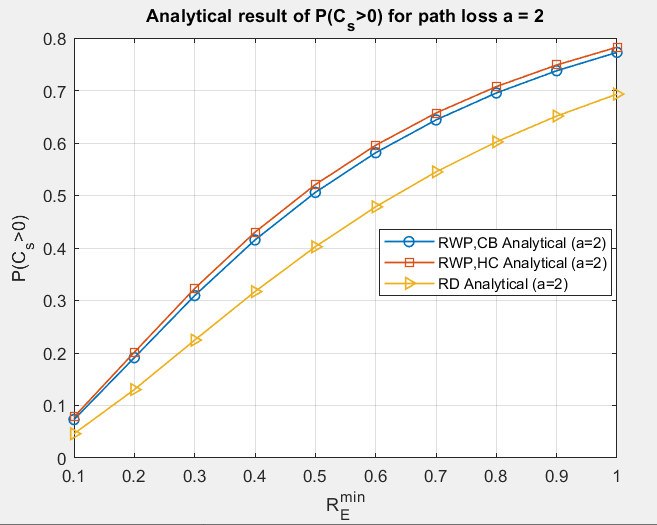
\includegraphics[width=0.9\textwidth]{PSCP_a_2.PNG} % second figure itself
        \caption{Reproduced figure}
    \end{minipage}
\end{figure}
\end{itemize}\\


\begin{itemize}
\begin{figure}[htp]
    \centering
    \begin{minipage}{0.45\textwidth}
        \centering
        \includegraphics[width=0.9\textwidth]{PSCP_4.PNG} % first figure itself
        \caption{Base Article figure}
    \end{minipage}\hfill
    \begin{minipage}{0.45\textwidth}
        \centering
        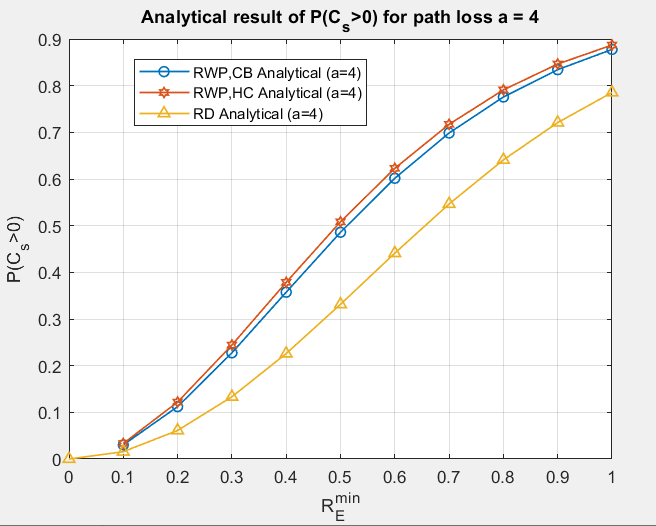
\includegraphics[width=0.9\textwidth]{PSCP_a_4.PNG} % second figure itself
        \caption{Reproduced figure}
    \end{minipage}
\end{figure}
\end{itemize}\\



\begin{itemize}
\begin{figure}[htp]
    \centering
    \begin{minipage}{0.45\textwidth}
        \centering
        \includegraphics[width=0.9\textwidth]{SOP_2.PNG} % first figure itself
        \caption{Base Article figure}
    \end{minipage}\hfill
    \begin{minipage}{0.45\textwidth}
        \centering
        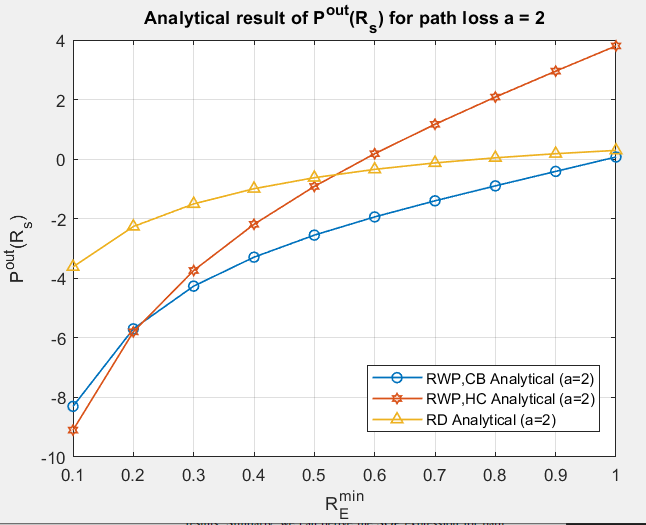
\includegraphics[width=0.9\textwidth]{SOP_a_2.PNG} % second figure itself
        \caption{Reproduced figure}
    \end{minipage}
\end{figure}
\end{itemize}\\


\begin{itemize}
\begin{figure}[htp]
    \centering
    \begin{minipage}{0.45\textwidth}
        \centering
        \includegraphics[width=0.9\textwidth]{SOP_4.PNG} % first figure itself
        \caption{Base Article figure}
    \end{minipage}\hfill
    \begin{minipage}{0.45\textwidth}
        \centering
        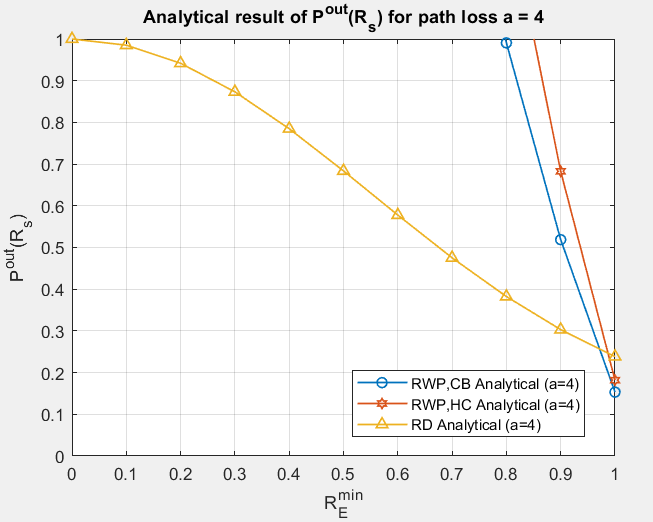
\includegraphics[width=0.9\textwidth]{SOP_a_4.PNG} % second figure itself
        \caption{Reproduced figure}
    \end{minipage}
\end{figure}
\end{itemize}
\newpage
\subsection{New Results}
\begin{itemize}
\item New Result\\
\begin{figure}[htp]
        \centering
        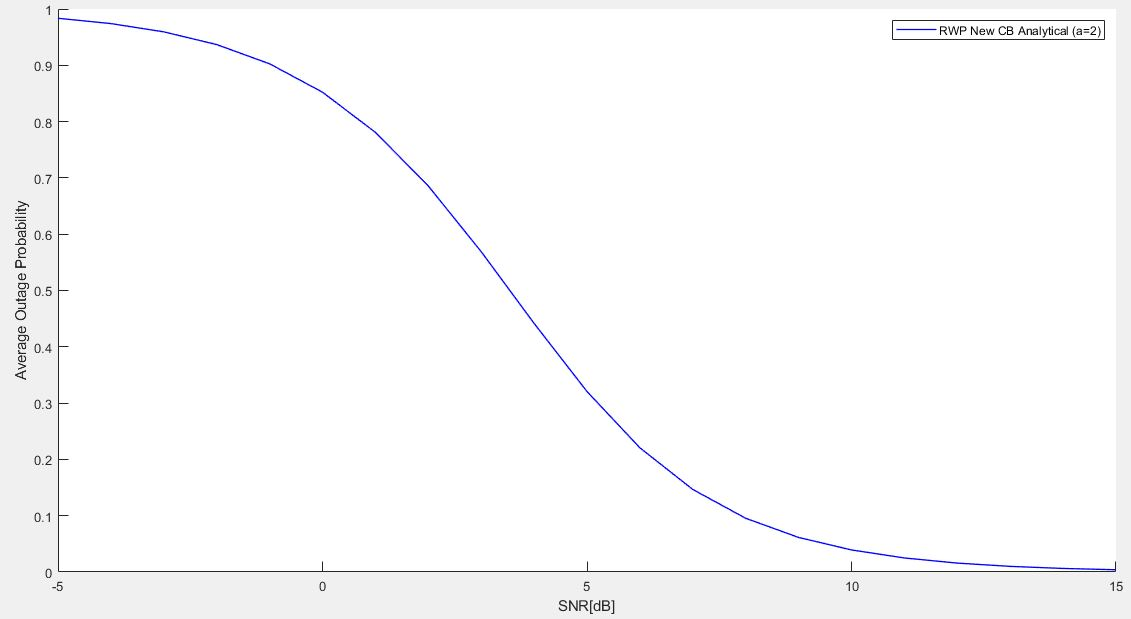
\includegraphics[width=12cm]{new_2.JPG}
        \caption{New Analysis}
        \label{fig:my_label}
    \end{figure}
\end{itemize}

	
\section{Conclusions}
	
\begin{itemize}
	
\item In the existing article, only Bob was moving and Eavesdropper was static. But as soon as the mobility of Eavesdropper was considered the Positive Secrecy Capacity Probability on user's side gets better.
Also impact of mobility will be seen on Secrecy outage probability. Secrecy Rate of user will be increased. 
\end{itemize}


\section{ Contribution of team members}	
\subsection{Technical contribution of all team members }
 \\
\begin{table}[h]
\centering
\begin{tabular}{|l|l|l|l|l|l|}
\hline
\textbf{Tasks} & \textbf{Shyam Patel} & \textbf{Ratnam Parikh} & \textbf{Dhairya Dudhatra} & \textbf{Jinesh Patel} & \textbf{Nisarg Shah} \\ \hline
Existing Derivation      &                       &         Y               &          &                        &         Y                             \\ \hline
Analytical       &     Y                   &                        &    Y      &       Y                 &                                      \\ \hline
Simulation          &      Y                  &                        &    Y      &        Y                &                                      \\ \hline
New Derivation        &                        &                 Y       &          &                        &      Y                                \\ \hline
New Analytical        &   Y                     &                        &      Y    & Y                       &                                      \\ \hline
\end{tabular}
\end{table}
\newpage

\subsection{Non-Technical contribution of all team members }

\begin{table}[h]
\centering
\begin{tabular}{|l|l|l|l|l|l|}
\hline
\textbf{Tasks} & \textbf{Shyam Patel} & \textbf{Ratnam Parikh} & \textbf{Dhairya Dudhatra} & \textbf{Jinesh Patel} & \textbf{Nisarg Shah} \\ \hline

Report          &         Y               &             Y           &   Y       &  Y                      &                 Y                     \\ \hline
Paper Reading         &    Y                    &                   Y     & Y         & Y                       &           Y                           \\ \hline
Brain Storming         & Y                       &                      Y  &    Y      &    Y                    &          Y                            \\ \hline
\end{tabular}
\end{table}

%\bibliographystyle{IEEEtran}
\newline
\section{References}
\newline
[1] A. D. Wyner, “The wire-tap channel,” Bell. Syst. Tech. J.,
vol. 54, no. 8, pp. 1355–1387, Oct. 1975.\newline
[2] M. Bloch, J. Barros, M. R. D. Rodrigues, and S. W. McLaugh-
lin, “Wireless information-theoretic security,” IEEE Trans. Inf.
Theory, vol. 54, no. 6, pp. 2515–2534, Jun. 2008.\newline
[3] X. Zhou, M. R. McKay, B. Maham, and A. Hjorungnes, “Re-
thinking the secrecy outage formulation: A secure transmission
design perspective,” IEEE Commun. Letter, vol. 15, no. 3, pp.
302–304, Mar. 2011. \newline
[4] J. Bai, X. Tao, J. Xu, and Q. Cui, “The secrecy outage proba-
bility for the ith closest legitimate user in stochastic networks,”
IEEE Commun. Letter, vol. 18, no. 7, pp. 1230–1233, Jul. 2014. \newline
[5] D. S. Karas, A. A. Boulogeorgos, and G. K. Karagiannidis,
“Physical layer security with uncertainty on the location of the
eavesdropper,” IEEE Wireless. Commun. Letter, vol. 5, no. 5,
pp. 540–543, Oct. 2016.\newline
[6] W. Liu, Z. Ding, T. Ratnarajah, and J. Xue, “On ergodic secrecy
capacity of random wireless networks with protected zones,”
IEEE Trans. Veh. Technol, vol. 65, no. 8, pp. 6146–6158, Aug.
2016.\newline
[7] X. X. L. Tao, Z. Yan and Z. Shidong, “Mean physical-layer
secrecy capacity in mobile communication systems,” Journal of
Tsinghua University, vol. 55, no. 11, pp. 1241–1245, 2015. \newline
[8] J. Wang, J. Lee, and T. Q. S. Quek, “Best antenna placement
for eavesdroppers: Distributed or co-located?” IEEE Commun.
Letter, vol. 20, no. 9, pp. 1820–1823, Sept. 2016. \newline
[9] T. X. Zheng, H. M. Wang, and Q. Yin, “On transmission
secrecy outage of a multi-antenna system with randomly located
eavesdroppers,” IEEE Commun. Lette, vol. 18, no. 8, pp. 1299–
1302, Aug. 2014. \newline
[10] H. Wang, X. Zhou, and M. C. Reed, “Physical layer security
in cellular networks: A stochastic geometry approach,” IEEE
Trans. Wireless Commun., vol. 12, no. 6, pp. 2776–2787, Jun.
2013. \newline
[11] K. Govindan, K. Zeng, and P. Mohapatra, “Probability density
of the received power in mobile networks,” IEEE Trans. Wire-
less Commun., vol. 10, no. 11, pp. 3613–3619, Nov. 2011.\newline
[12] C. Bettstetter, H. Hartenstein, and X. P. Costa, “Stochastic
properties of the random waypoint mobility model,” Wireless
Networks, vol. 10, no. 5, pp. 555–567, 2004.\newline
[13] P. Nain, D. Towsley, B. Liu, and Z. Liu, “Properties of random
direction models,” in IEEE INFOCOM, vol. 3, Mar. 2005, pp.
1897–1907 vol. 3.\newline
[14] V. A. Aalo, C. Mukasa, and G. P. Efthymoglou, “Effect of
mobility on the outage and ber performances of digital trans-
missions over Nakagami-m fading channels,” IEEE Trans. Veh.
Technol, vol. 65, no. 4, pp. 2715–2721, Apr. 2016.\newline
[15] E. Hyytia, P. Lassila, and J. Virtamo, “Spatial node distribution
of the random waypoint mobility model with applications,”
IEEE Trans. Mobile Comput., vol. 5, no. 6, pp. 680–694, Jun.
2006.\newline
%\bibliography{ref.bib}


\end{document} 